%%%%%%%%%%%%%%%%%%%%%%% file template.tex %%%%%%%%%%%%%%%%%%%%%%%%%
%
% This is a general template file for the LaTeX package SVJour3
% for Springer journals.          Springer Heidelberg 2010/09/16
%
% Copy it to a new file with a new name and use it as the basis
% for your article. Delete % signs as needed.
%
% This template includes a few options for different layouts and
% content for various journals. Please consult a previous issue of
% your journal as needed.
%
%%%%%%%%%%%%%%%%%%%%%%%%%%%%%%%%%%%%%%%%%%%%%%%%%%%%%%%%%%%%%%%%%%%
%
% First comes an example EPS file -- just ignore it and
% proceed on the \documentclass line
% your LaTeX will extract the file if required
\begin{filecontents*}{example.eps}
%!PS-Adobe-3.0 EPSF-3.0
%%BoundingBox: 19 19 221 221
%%CreationDate: Mon Sep 29 1997
%%Creator: programmed by hand (JK)
%%EndComments
gsave
newpath
  20 20 moveto
  20 220 lineto
  220 220 lineto
  220 20 lineto
closepath
2 setlinewidth
gsave
  .4 setgray fill
grestore
stroke
grestore
\end{filecontents*}
%
\RequirePackage{fix-cm}
%
%\documentclass{svjour3}                     % onecolumn (standard format)
%\documentclass[smallcondensed]{svjour3}     % onecolumn (ditto)
\documentclass[smallextended]{svjour3}       % onecolumn (second format)
%\documentclass[twocolumn]{svjour3}          % twocolumn
%
\smartqed  % flush right qed marks, e.g. at end of proof
%
\usepackage{graphicx}
\usepackage[numbers]{natbib}
\usepackage{bussproofs}
\usepackage{amsmath}
\usepackage{tikz}
\usetikzlibrary{positioning}
\usetikzlibrary{decorations.pathmorphing}

\tikzset{snake it/.style={decorate, decoration=snake}}

\usepackage[T1]{fontenc}
\DeclareFontFamily{T1}{calligra}{}
\DeclareFontShape{T1}{calligra}{m}{n}{<->s*[1.44]callig15}{}
\DeclareMathAlphabet\mathzapf       {T1}{pzc} {mb} {it}


%
% \usepackage{mathptmx}      % use Times fonts if available on your TeX system
%
% insert here the call for the packages your document requires
%\usepackage{latexsym}
% etc.
%
% please place your own definitions here and don't use \def but
% \newcommand{}{}
%
% Insert the name of "your journal" with
% \journalname{myjournal}
%
\begin{document}


\title{(Parallel) Efficient Subclasses Of CFL-Reachability Queries%\thanks{Grants or other notes
%about the article that should go on the front page should be
%placed here. General acknowledgments should be placed at the end of the article.}
}
%\subtitle{Do you have a subtitle?\\ If so, write it here}

%\titlerunning{Short form of title}        % if too long for running head

\author{Ekaterina Shemetova         \and
        Semyon Grigorev %etc.
}

%\authorrunning{Short form of author list} % if too long for running head

\institute{E. Shemetova \at
             St. Petersburg Academic University, ul. Khlopina, 8, Saint Petersburg 194021, Russia \\
              \email{katyacyfra@gmail.com}           %  \\
%             \emph{Present address:} of F. Author  %  if needed
           \and
           S. Grigorev \at
              St. Petersburg State University, 7/9 Universitetskaya nab., Saint Petersburg 199034, Russia \\
              \email{rsdpisuy@gmail.com}    
}

\date{Received: date / Accepted: date}
% The correct dates will be entered by the editor


\maketitle

\begin{abstract}
The context-free language (CFL) reachability problem for a context-free grammar $G$ and directed edge-labelled graph $D$ consists of determining for every pair of nodes  $v$ and $u$ whether $v$ can reach $u$ via a path labelled by string in $L(G)$. 
\par
Inspite the 
\keywords{CFL-reachability \and Complexity \and Boolean circuit}
% \PACS{PACS code1 \and PACS code2 \and more}
% \subclass{MSC code1 \and MSC code2 \and more}
\end{abstract}



\section{Introduction}
\label{intro}
The context-free language (CFL) reachability problem is an important problem underlying some fundamential static code analyses \cite*{RepsBasic, Incremental} and graph database query evaluation \cite{HellingsCFPQ}\cite{RDF}\cite{GrigorevRagozina}.
\par
Unlike context-free language recognition, which is in NC, CFL-reachability is P-complete \cite{Yannakakis}\cite{RepSeq}. Practically, it means that we don't have an efficient parallel algorithm for solving this problem (unless $P \neq NC$). But want some cases... . Simple cases (examples, trees etc)... Our focus is on the...
\\This paper is organized as follows.
\section{Preliminaries}
\label{sec:prel}
\label{preliminaries}
\paragraph{CFL-reachability} 
The general formulation of CFL-reachability problem can be stated as follows.
\\$l(\pi)$ denotes a string which is obtained from concatenation of edge labels of the path $\pi$.
\paragraph{Circuits and complexity classes} 
\paragraph{General complexity of CFL-reachability} It is well known that CFL-reachability problem is P-complete \cite{Yannakakis}. 
\section{Boolean circuit}
\label{sec:circuit}
In this section we build generalization of classical Boolean circuit for context-free recognition from the Brent-Goldschlager-Rytter algorithm \cite*{Brent, Rytter} in order to evaluate CFL-reachability problem.
\subsection{Circuit description}
\label{Bdesc}
The idea of the Brent-Goldschlager-Rytter parallel algorithm is based on replacement of ordinary parse trees with a equivalent system of logical dependencies. We can adapt this system for graph input as follows (context-free grammar is in the Chomsky normal form):
\begin{enumerate}
\item $\frac{i \xrightarrow{a} j}{A(i , j)}$  --- if edge from the node $i$ to the node $j$ has label "$a$" and $A \rightarrow a \in P$, then there is a parse tree with nonterminal $A$ at the root deriving a path from $i$ to $j$.
\\
\item $\frac{B(i , j)}{\frac{A}{C}(i , j :: z)}$ --- creating a gap on the right: if a parse tree with the nonterminal $B$ at the root deriving a path from $i$ to $j$ exists and $A \rightarrow BC \in P$, then a parse tree with nonterminal $A$ at the root containing a smaller subtree with the nonterminal $C$ deriving path from $j$ to $z$ ("gap"), where $1 \le z \le n$, may exist.
\\
\item $\frac{C(j  , z)}{\frac{A}{B}(i :: j  , z)}$ --- creating a gap on the left: if a parse tree with the nonterminal $C$ at the root deriving a path from $j$ to $z$ exists and $A \rightarrow BC \in P$,  then a parse tree with nonterminal $A$ at the root containing a smaller subtree with the nonterminal $B$ deriving a path from $i$ to $j$ ("gap"), where $1 \le i \le n$, may exist.
\\
\item  $\frac{B(i, j), \frac{A}{B}(i :: j  , z)}{A(i, z)}$ --- filling the gap: if a parse tree with the nonterminal $A$ at the root deriving a path from $i$ to $z$, which cointains the gap represented by a node labelled $B$ deriving a path from $i$ to $j$ and a parse tree with the nonterminal $B$ at the root deriving a path from $i$ to $j$ exist, then the whole parse tree with the nonterminal $A$ at the root deriving a path from $i$ to $z$ exists.
\\
\item $\frac{\frac{A}{E}(i , j :: w, z), \frac{E}{D}( j , u :: v , w)}{\frac{A}{D}(i, u :: v , z)}$ --- combination of conditional propositions: if there is a parse tree with the nonterminal $A$ at the root deriving a path from $i$ to $z$ with the gap represented by a node labelled $E$ deriving a path from $j$ to $w$ and there is a parse tree with the nonterminal $E$ at the root deriving a path from $j$ to $w$, which contains gap represented by some node $D$, then there is a parse tree with the nonterminal $A$ at the root deriving a path from $i$ to $z$, which contains the gap represented by the above mentioned node $D$.
\end{enumerate}


Using logical dependencies above, elements of the circuit can be described with two types of elements: $x_{A, i,  j}$, which is true when a parse tree with the nonterminal $A$ at the root deriving a path from $i$ to $j$ exists, and $y_{A, i,  j, B, k, l}$ for conditional propositions, which is true when there is a parse tree with the nonterminal $A$ at the root deriving a path from $i$ to $j$ containg a hole instead of a subtree with the nonterminal $B$ at the root deriving a path from $k$ to $l$.


Therefore the circuit contains the following gates:
\begin{itemize}
\item \textit{Input}: input gates, one gate for every edge of the input graph and alphabet symbol; evaluates to true if the corresponding edge has an appropriate label
\item internal AND-gates for evaluating the combinations of conditional propositions and filling the gaps
\item internal OR-gates for creating gaps: conditional proposition $y_{A, i,  j, E, k, l}$ can be obtained by taking the gap from the right subtree (if $x_{B, i,  z}$ is true and $y_{C, z,  j, E, k, l}$ is true) or by taking the gap from the left subtree ($y_{B, i,  z, E, k, l}$ is true and $x_{C, z,  j}$ is true) for rule $A \rightarrow BC \in P$ . Notice that if start and end nodes of the tree with the gap coincide with start and end nodes of the gap ($i = k, z = l$ for the left case, $z = k, j = l$ for the right case), then the gap just added to the left or right side of another tree.
\item  \textit{Output}: output gates, one gate for every pair of graph nodes and nonterminal; evaluates to true if appropriate parse tree exists.
\end{itemize}

\subsection{Bounds on the circuit size and depth}
\paragraph{Circuit size}
\begin{lemma}
Let $G = (\Sigma, N, P)$ be a context-free grammar in Chomky normal form and let $n$ be a number of nodes in the input graph. Then the circuit described in \ref{Bdesc} has $O(n^6)$ elements.
\end{lemma}
\begin{proof} Let's count circuit gates by type. The number of input gates is $|\Sigma|n^2$ and the number of output gates is $|N|n^2$. Also there are $|N|^2n^5$ OR-gates for creating the gaps and $|N|^2n^4$ AND-gates for filling gaps. It is easy to see that the maximal number of elements is needed for combinations of conditional propositions: there are $|N|^3n^6$ such elements ( $|N|^2n^4 \times |N|n^2$ ). Therefore the circuit contains at most $O(n^6)$ elements.
\end{proof}
\paragraph{Circuit depth}
Before we analyze the depth of the circuit we shall prove the following statement.
\begin{lemma}
\label{bigsubtree}
Let $G = (\Sigma, N, P)$ be a context-free grammar in Chomky normal form. Then every parse tree with $k$ leaves contains a middle node ("critical" node) that spans over more than $\frac{1}{3}k$ and at most $\frac{2}{3}k$ leaves.
\end{lemma}
\begin{proof} Because the grammar is in the Chomsky normal form, every node of a parse tree has two children. Going from the root to leaves, we can choose the largest of two subtrees at each node while the current subtree has more than $\frac{2}{3}k$ leaves. Obviously, the first node that has at most $\frac{2}{3}k$ leaves is bound to have more than $\frac{1}{3}k$ leaves due to binary branching. 
\end{proof}
\begin{lemma}
\label{depthproof}
Let $l$ be a length of the shortest path from node $i$  to node $j$ labelled by string from $L(G_A)$. Then proposition $A(i, j)$ or $\frac{A}{D}(i , u :: v, j)$ has a proof of height $O(\log l)$.
\end{lemma}
\begin{proof} Proof by induction on $l$.
\\ \textit{Induction hypotesis}: every proposition with no more than $\frac{2}{3}l$ leaves has a proof of logarithmic height ($O(\log l)$).


At first, consider the proposition $A(i, j)$. By Lemma \ref{bigsubtree}, a corresponding tree has a critical node $E$ with two children $B$ and $C$ (for $E \rightarrow BC \in P$). Then we can write the proof tree as follows.
\begin{prooftree}
\AxiomC{$B(u, l)$}
\AxiomC{$C(l, v)$}
\BinaryInfC{$E(u, v)$}
\AxiomC{$\frac{A}{E}(i , u :: v , j)$}
\BinaryInfC{$A (i, j)$}
\end{prooftree}
Because $E$ is the critical node, each of the propositions $B(u, l), C(l, v)$, $\frac{A}{E}(i , u :: v , j)$ has no more than $\frac{2}{3}l$ leaves and therefore has a proof of logarithmic height by inductive hypothesis.


There are two cases for the second proposition $\frac{A}{D}(i , u :: v, j)$.

\begin{figure}
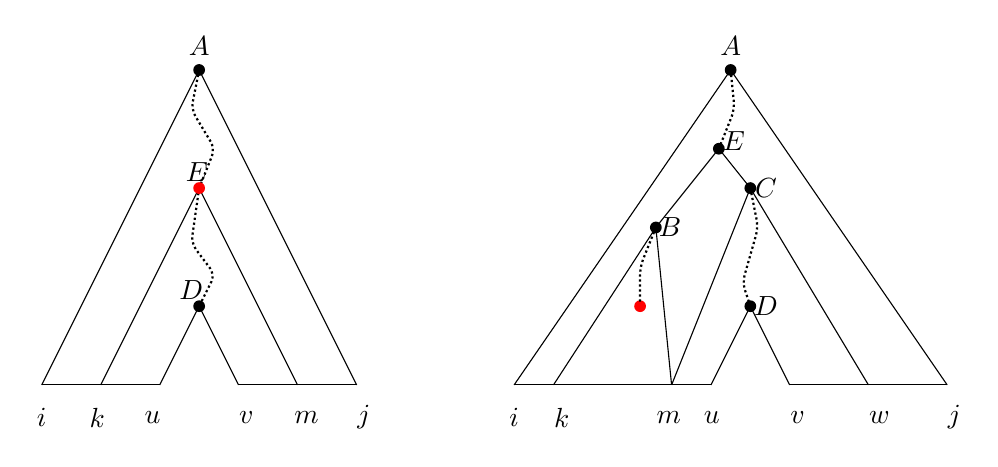
\begin{tikzpicture}
\draw (0,0) -- (1.5,0) ;
\draw (0,0) -- (2,4) ;
\draw (2,4) -- (4,0) ;
\draw (1.5,0) -- (2,1) ;
\draw (2,1) -- (2.5,0) ;
\draw (2.5,0) -- (4,0) ;
\draw (0.75,0) -- (2,2.5) ;
\draw (2,2.5) -- (3.25,0) ;
\draw [thick,densely dotted, rounded corners=1mm](2,4) --  (1.9, 3.5) -- (2.2, 3) -- (2,2.5);
\draw [thick,densely dotted, rounded corners=1mm] (2,2.5) -- (1.9, 1.8) -- (2.2, 1.4) -- (2,1);
\node (start) {}; 
\node [below=0.05cm of start] (i1) {$i$};
\node [right=3.7cm of i1] (j1) {$j$}; 
\node [right=0.3cm of i1] (k1) {$k$}; 
\node [right=1cm of i1] (u1) {$u$}; 
\node [right=2.2cm of i1] (v1) {$v$}; 
\node [right=2.9cm of i1] (m1) {$m$}; 
\node [right=2.0cm of start] (middle1) {}; 
\node (A1) at (2, 4.3) {$A$}; 
\node (D1) at (1.9, 1.2) {$D$};
\node [circle, fill=red, inner sep = 1.5pt, minimum size=1pt](cr) at (2, 2.5) {};
\node (E1) at (1.97, 2.7) {$E$};
\node [circle, fill=black, inner sep = 1.5pt, minimum size=1pt](pD1) at (2,1) {};
\node [circle, fill=black, inner sep = 1.5pt, minimum size=1pt](pA1) at (2,4) {};

%second picture
\draw (6,0) -- (8.5,0) ;
\draw (9.5,0) -- (11.5,0) ;
\draw (6,0) -- (8.75,4) ;
\draw (8.75,4) -- (11.5,0) ;
%\draw (7,0) -- (8.8,3) ;
%\draw (8.8,3) -- (10.5,0) ;
\draw (8.5,0) -- (9,1) ;
\draw (9,1) -- (9.5,0) ;
\draw (6.5, 0) -- (7.8,2) ;
\draw (7.8,2) -- (8,0) ;
\draw (8,0) -- (9,2.5) ;
\draw (9,2.5) -- (10.5,0) ;
\draw (8.6,3) -- (9,2.5) ;
\draw (8.6,3) -- (7.8,2) ;
\node (start2) at (6, 0) {}; 
\node [below=0.05cm of start2] (i2) {$i$};
\node [right=0.2cm of i2] (k2) {$k$}; 
\node [right=1.5cm of i2] (m2) {$m$}; 
\node [right=2.1cm of i2] (u2) {$u$}; 
\node [right=3.2cm of i2] (v2) {$v$}; 
\node [right=4.2cm of i2] (w) {$w$}; 
\node [right=5.2cm of i2] (j2) {$j$}; 
\node (A2) at (8.75, 4.3) {$A$}; 
\node (E2) at (8.79, 3.1) {$E$}; 
\node (B) at (7.98, 2) {$B$}; 
\node (C) at (9.2,2.5) {$C$}; 
\node (D2) at (9.2,1) {$D$}; 
\node [circle, fill=black, inner sep = 1.5pt, minimum size=1pt](pB) at (7.8,2) {};
\node [circle, fill=red, inner sep = 1.5pt, minimum size=1pt](crU) at (7.6,1) {};
\node [circle, fill=black, inner sep = 1.5pt, minimum size=1pt](pA2) at (8.75,4) {};
\node [circle, fill=black, inner sep = 1.5pt, minimum size=1pt](pC) at (9,2.5) {};
\node [circle, fill=black, inner sep = 1.5pt, minimum size=1pt](pE2) at (8.6,3) {};
\node [circle, fill=black, inner sep = 1.5pt, minimum size=1pt](pD2) at (9,1) {};
\draw [thick,densely dotted, rounded corners=1mm](9,2.5) -- (9.1, 2) -- (8.9, 1.3) -- (9,1) ;
\draw [thick,densely dotted, rounded corners=1mm](8.75,4) -- (8.8, 3.5) -- (8.6,3);
\draw [thick,densely dotted, rounded corners=1mm]  (7.8,2) -- (7.6, 1.5) -- (7.6,1.05);
\end{tikzpicture}
% Use the relevant command to insert your figure file.
% For example, with the graphicx package use
% figure caption is below the figure
\caption{ Cases for conditional proposition $\frac{A}{D}(i , u :: v, j)$: (left) a subtree with the critical node at the root contains the hole; (right) a subtree with the critical node at the root contains only leaves corresponding to the path $i \rightarrow u$.}
\label{proofcases}       % Give a unique label
\end{figure}



\begin{enumerate}
\item \textit{A subtree with the critical node at the root contains the hole $u :: v$.} 
\\ Let $E$ be a label of the critical node. Then a corresponding subtree splits the path from the vertex $i$ to the vertex $u$ onto two paths: $i \rightarrow k$ and $k \rightarrow u$ and the path from the vertex $v$ to the vertex $j$ onto $v \rightarrow m$ and $m \rightarrow j$ respectively (as illustrated in Figure \ref{proofcases}(left)). The next proof tree represents the proof of the proposition $\frac{A}{D}(i , u ::v, j)$ in this case. 
\begin{prooftree}
\AxiomC{$\frac{A}{E}(i , k :: m , j)$}
\AxiomC{$\frac{E}{D}(k , u :: v , m)$}
\BinaryInfC{ $\frac{A}{E}(i , u :: v , j)$}
\end{prooftree}
Conditional proposition $\frac{A}{E}(i , k :: m , j)$ and $\frac{E}{D}(k , u :: v , m)$ have no more than $\frac{2}{3}l$ leaves, so $\frac{A}{E}(i , u :: v , j)$ has a proof of logarithmic height.

\item \textit{A subtree with the critical node at the root contains only leaves corresponding to the path from the vertex $i$ to the vertex $u$ in the input graph.}


This case is illustrated in Figure \ref{proofcases}(right). Consider the biggest subtree which contains a subtree with the critical node at the root and has leaves corresponding only to the path from the vertex $i$ to the vertex $u$ of the input graph. Let $B$ be a label at the root of this tree and $k \rightarrow m$  be a corresponding path in the input graph. Let $E$ be a parent node of node $B$ and let $C$ be a second child of $E$ (for $E \rightarrow BC \in P$). A parse tree with the root labelled by $C$ has some leaves corresponding to the path $v \rightarrow j$, so let $w$ be a vertex which splits this path on two. Now we are able to write the proof of $\frac{A}{E}(i , u :: v , j)$.
\begin{prooftree}
\AxiomC{$\frac{A}{E}(i , k :: w , j)$}
\AxiomC{$B(k, m)$}
\UnaryInfC{$\frac{E}{C}(k , m :: w)$}
\AxiomC{$\frac{C}{D}(m , u :: v , w)$}
\BinaryInfC{$\frac{E}{D}(k , u ::v , w)$}
\BinaryInfC{ $\frac{A}{D}(i , u :: v , j)$}
\end{prooftree}
The subtree with the root labelled $B$ obviously contains at least $\frac{2}{3}l$ leaves, so each of the other propositions $\frac{C}{D}(m , u :: v , w)$ and $\frac{A}{E}(i , k :: w , j)$ has no more then  $\frac{2}{3}l$ leaves. By induction hypothesis they have a proof of logarithmic height. Thus, proposition  $\frac{A}{D}(i , u :: v , j)$ can be proved via 4 steps using propositions with the proofs of logarithmic depth.
\\The case when the subtree with the critical node at the root contains only leaves corresponding to the path from the vertex $v$ to the vertex $j$ in the input graph is held symmetrically.
\end{enumerate}
\end{proof}
Using lemmas above, we can conclude the following.
\begin{corollary}
\label{coldepth}
Let $G = (\Sigma, N, P)$ be a context-free grammar in Chomky normal form and let $\mathzapf{L}$ be the length of the maximum in all nonterminals and all pairs of graph nodes shortest path labelled by a string from $L(G)$. Then there is a uniform family of circuits for solving CFL-reachability problem on the graphs with $n$ nodes, which are of depth $O(\log n \log \mathzapf{L})$ and contain $O(n^6)$ elements.
\end{corollary}


The depth and therefore the efficiency of the circuit depends on the value of parameter $\mathzapf{L}$. We investigate bounds for $\mathzapf{L}$ in the next two sections.

\section{Efficient subclasses of context-free languages}
\label{sec:CF}
In this section our focus is on estimating the value of $\mathzapf{L}$ for some fixed context-free languages and arbitrary input graphs. 
\subsection{General case}
Hellings in \cite{HellingsCFPQ} gave the worst-case lower and upper bounds on the $\mathzapf{L}$ parameter.
\begin{theorem}[Hellings]
Let  $G = (\Sigma, N, P)$ be a context-free grammar and $D=(V, E, \Sigma)$ be a directed labelled graph with $n$ nodes. In the worst case, we have $ n^22^{|N|}\le \mathzapf{L} \le 2^{|N|n^2-1}$.
\end{theorem}


Using the bounds above and Corollary \ref{coldepth}, we can get the maximum depth of our circuit in the worst case: 
$O(\log n \log \mathzapf{L}) = O(\log n \log 2^{|N|n^2-1}) = \\ = O(|N|n^2\log n)$. The circuit can have a depth which is polynomial on the input length in case of arbitrary context-free grammar. It is not surprising because of the nature of P-completeness: we don't have an efficient parallel algorithm or circuit with a polylogarithmic on the input length depth for CFL-reachability problem because it is P-complete problem (unless $P \neq NC$).


But we also have a polynomial lower bound on $\mathzapf{L}$, which give us the effective circuit with depth $O(\log^2 n)$. Our next goal is to investigate important subclasses of context-free languages, and find those for which CFL-reachability is in the class $NC$.
\subsection{Rational index}
It is known that the value of $\mathzapf{L}$ is different for various types of context-free languages, in particular it can be bounded from above by the polynomial or exponential function on the number of graph nodes \cite*{Dyck1, CFRat, GreibRat}. Boasson et al. in \cite{RatBasic} introduced definition of such function called \textit{rational index}. For a language $L$ on an alphabet $\Sigma$, its rational index $\rho_L$ is a function defined as follows:
\begin{equation}
\rho_L(n) = \max\{\min\{|w|:w \in L \cap K\}, K \in {Rat}_n, L \cap K \neq \emptyset\},
\end{equation} where $|w|$ is the length of a word $w$ and ${Rat}_n$ denotes the set of regular languages on an alphabet $\Sigma$, recognized by a finite nondeterministic automation with at most $n$ states.


It is easy to see that in the case of fixed context-free language and arbitrary graph, $\mathzapf{L}$ is some kind of the rational index: we can represent arbitrary graphs with $n$ nodes via nondeterministic automations with at most $n$ states, then $\mathzapf{L}$ is exactly rational index. So, we have the following corollary.
\begin{corollary}
\label{ratdepth}
Let $L$ be a context-free language on an alphabet $\Sigma$, which has a polynomially bounded from above rational index, and $D=(V, E, \Sigma)$ be a directed labelled graph with $n$ nodes. Then, CFL-reachability problem for $L$ and $D$ is in $NC^2$.
\end{corollary}
\subsection{Linear languages}
\begin{figure}
\begin{tikzpicture}
\node{S}
 child {node {a}}
 child {node {$A$} 
      child {node {b}}
      child { node {$B$}
        child { node {$C$}
                     child {node {d}}
                     child { node {$...$}} }
        child { node {$c$}} }
     };
\end{tikzpicture}
% Use the relevant command to insert your figure file.
% For example, with the graphicx package use
% figure caption is below the figure
\caption{A parse tree for linear grammar in the Chomsky normal form.}
\label{ptlin}       % Give a unique label
\end{figure}
A \textit{linear language} is a language generated by some \textit{linear grammar}. A \textit{linear grammar} is a context-free grammar that has at most one nonterminal in the right hand side of each of its productions. The linear grammar  $G = (\Sigma, N, P)$ is said to be in the Chomsky normal form, when all of its production rules are of the form: $A \rightarrow aB$, or $A \rightarrow Ba$, or $A \rightarrow a$, where $B \in N$ and $a \in \Sigma$.


Before we consider the value of $\mathzapf{L}$ for linear grammars, we shall prove the following.
\begin{lemma}
\label{lem:treeheight}
Let  $G = (\Sigma, N, P)$ be a context-free grammar,  $D=(V, E, \Sigma)$ be a directed labelled graph with $n$ nodes and $\pi$ be the maximum in all nonterminals and all pairs of graph nodes shortest path labelled by a string from $L(G)$. Then a height of a parse tree for $l(\pi)$ does not exceed $|N|n^2$.
\end{lemma}

\begin{proof}
 Assume that the parse tree for $l(\pi)$ has a height of more than $|N|n^2$. There are $|N|n^2$ unique labels $(A, i, j)$ for nodes of the parse tree, so according to the pigeonhole principle, the parse tree for $l(\pi)$ contains at least one subtree $T$ with label $(A, i, j)$ at the root, which has a subtree $T'$ with the same label. Then we can change $T$ with $T'$ and get a new string $l(\pi')$ which is shorter than $l(\pi)$. But $l(\pi)$ is the shortest, then we have a contradiction.

\end{proof}
\begin{theorem}
\label{thlin}
Let  $G = (\Sigma, N, P)$ be a linear grammar and $D=(V, E, \Sigma)$ be a directed labelled graph with $n$ nodes. Then the length of the maximum in all nonterminals and all pairs of graph nodes shortest path labelled by a string from $L(G)$ ($\mathzapf{L}$) is $O(|N|n^2)$.
\end{theorem}

\begin{proof}
From Lemma \ref{lem:treeheight}, a height of a parse tree is no more then $|N|n^2$. Let's construct a parse tree of such height for linear grammar in the Chomsky normal form. Every rule for linear grammar has at most one nonterminal in the right hand side of each of its productions, so if the grammar is in the Chomsky normal form, then there is the only one terminal symbol at the every level of the parse tree (as illustrated in Figure \ref{ptlin}). The tree has no more then $|N|n^2$ levels, so the length of any shortest path labelled by a string from $L(G)$ is no more than $O(|N|n^2)$.
\end{proof}
Combining Theorem \ref{thlin} and Corollary \ref{coldepth} we are able to conclude the following.
\begin{corollary} 
Let  $G = (\Sigma, N, P)$ be a linear grammar and $D=(V, E, \Sigma)$ be a directed labelled graph with $n$ nodes. Then CFL-reachability problem for $G$ and $D$ is in $NC^2$.
\end{corollary}

\subsection{Dyck languages}
\textit{Dyck language over $\Sigma_k$} is the set of well-balanced words over alphabet $\Sigma_k = \{(_1, (_2, ..., (_k, )_1, )_2, ..., )_k\}$. Dyck language can be defined by the following rules:
\\$S \rightarrow SS$ | $S \rightarrow \varepsilon$ |$S \rightarrow (_1S)_1$ | $S \rightarrow (_2S)_2$ | ... | $S \rightarrow (_kS)_k$, where $S$ is the start symbol, and $\varepsilon$ is the empty string. We will denote the Dyck language over $\Sigma_i$ by $D_i$.


Dyck languages play an important role in formal languages theory. The famous Chomsky-Sch\"utzenberger theorem states that every context-free language $L$ can be represented via a regular language $R$ and a Dyck language $D_n$, which are combined by means of an intersection and a homomorphism $h$. 
\begin{equation}
L = h(D_n \cap R)
\end{equation}


Because every context-free language can be represented with Dyck language, it is natural to expect that CFL-reachability is P-complete for Dyck languages. P-completeness for the similiar problem LGAP in case of $D_2$ was proved in \cite*{PCompl, LReach, Regularrealizability}. We will show that $\mathzapf{L}$ is exponential for $D_k$ where $k\ge2$, so our circuit is not effective in that case.
\begin{lemma}[Pierre]
\label{pierrelem}
The rational indexes of generators of context-free languages belongs to $exp(\Theta(n^2/\ln n))$.
\end{lemma}
\begin{theorem}
Let $L$ be a Dyck language over $k \ge 2$ brackets and $D=(V, E, \Sigma)$ be a directed labelled graph with $n$ nodes. Then, $\mathzapf{L}$  belongs to $exp(\Theta(n^2/\ln n))$.
\end{theorem}
\begin{proof}
By definition, generator is a context-free language which can transform into any context-free language through a rational transduction \cite{CFRat}.
Notice that for $k>2$ homomorphism $g$ such that $D_k = g^{-1}(D_2)$ can be constructed. Thanks to the Chomsky-Sch\"utzenberger theorem, we have the following equation.
\begin{equation}
L = h(g^{-1}(D_2)\cap R)
\end{equation}
Thus, every context-free language can be generated by $D_k$, where $k \ge 2$. By \ref{pierrelem} we can conclude that $\mathzapf{L}$ for $D_k$ belongs to $exp(\Theta(n^2/\ln n))$. 
\end{proof}

Notice that $D_1$ is not a generator of any context-free language. But it is known that $D_1$ is a generator of \textit{one-counter languages} \cite{GreibHier}. \textit{One-counter} languages are the languages recognized by \textit{one-counter automata} --- pushdown automata with a single stack symbol. 
\begin{lemma}[Deleage, Pierre]
\label{dyck1lem}
The rational index of $D_1$ is $O(n^2)$.
\end{lemma}
\begin{theorem}
\label{onecounter}
Let $L$ be a one-counter language, and $D=(V, E, \Sigma)$ be a directed labelled graph with $n$ nodes. Then, CFL-reachability problem for $L$ and $D$ is in $NC^2$.
\end{theorem}
\begin{proof} (Sketch)
Because $D_1$ is a generator of one-counter languages \cite{GreibHier}, every one-counter language can be represented by regular language $R$ and $D_1$, which are combined by means of an intersection and a homomorphism $h$. By Lemma \ref{dyck1lem}, $\mathzapf{L}$ for intersection of $D_1$ and $R$ stays polynomial, homomorphism operation doesn't change the polinomiality of $\mathzapf{L}$ too (?). Thus, by Corollary \ref{coldepth}, the depth of the circuit for one-counter languages is $O(\log^2 n)$.
\end{proof}


Notice that there is an effective sequential algorithm for CFL-reachability for $D_1$ based on matrix multiplication \cite{Bradford}. We propose that using Theorem \ref{onecounter} it can be extended for working with one-counter languages.

\subsection{Iterative property}





%\begin{acknowledgements}
%If you'd like to thank anyone, place your comments here
%and remove the percent signs.
%\end{acknowledgements}


% Authors must disclose all relationships or interests that 
% could have direct or potential influence or impart bias on 
% the work: 
%
% \section*{Conflict of interest}
%
% The authors declare that they have no conflict of interest.


% BibTeX users please use one of
%\bibliographystyle{spbasic}      % basic style, author-year citations
%\bibliographystyle{spmpsci}      % mathematics and physical sciences
%\bibliographystyle{spphys}       % APS-like style for physics
%\bibliography{}   % name your BibTeX data base

% Non-BibTeX users please use
%\begin{thebibliography}{}
%
% and use \bibitem to create references. Consult the Instructions
% for authors for reference list style.
%
%\bibitem{RefJ}
% Format for Journal Reference
%Author, Article title, Journal, Volume, page numbers (year)
% Format for books
%\bibitem{RefB}
%Author, Book title, page numbers. Publisher, place (year)
% etc
%\end{thebibliography}
\bibliographystyle{spbasic}      % basic style, author-year citations
\bibliography{article}   % name your BibTeX data base
\end{document}
% end of file template.tex

